\documentclass{article}
\usepackage{graphicx} % Required for inserting images
\usepackage[landscape, a4paper, margin=20pt]{geometry}
\usepackage{tikz}
\usetikzlibrary{shapes.geometric, arrows.meta, positioning}
\usepackage[version=4]{mhchem}
\usepackage{chemfig}
\usepackage[symbol]{footmisc}

\title{A synthesis flowchart for Edexcel International A-level Chemistry}
\author{ Bryan Li }
\date{\today}

\tikzset{rect/.style={rectangle, minimum width=2.5cm, text width=2.5cm, minimum height=1cm, text centered, draw=black, align=center}}
\tikzset{line/.style={thick, font=\small, >={Latex[length=3mm, width=2mm]}}}
\tikzset{arrow/.style={->, line}}

\begin{document}
\maketitle
\pagebreak
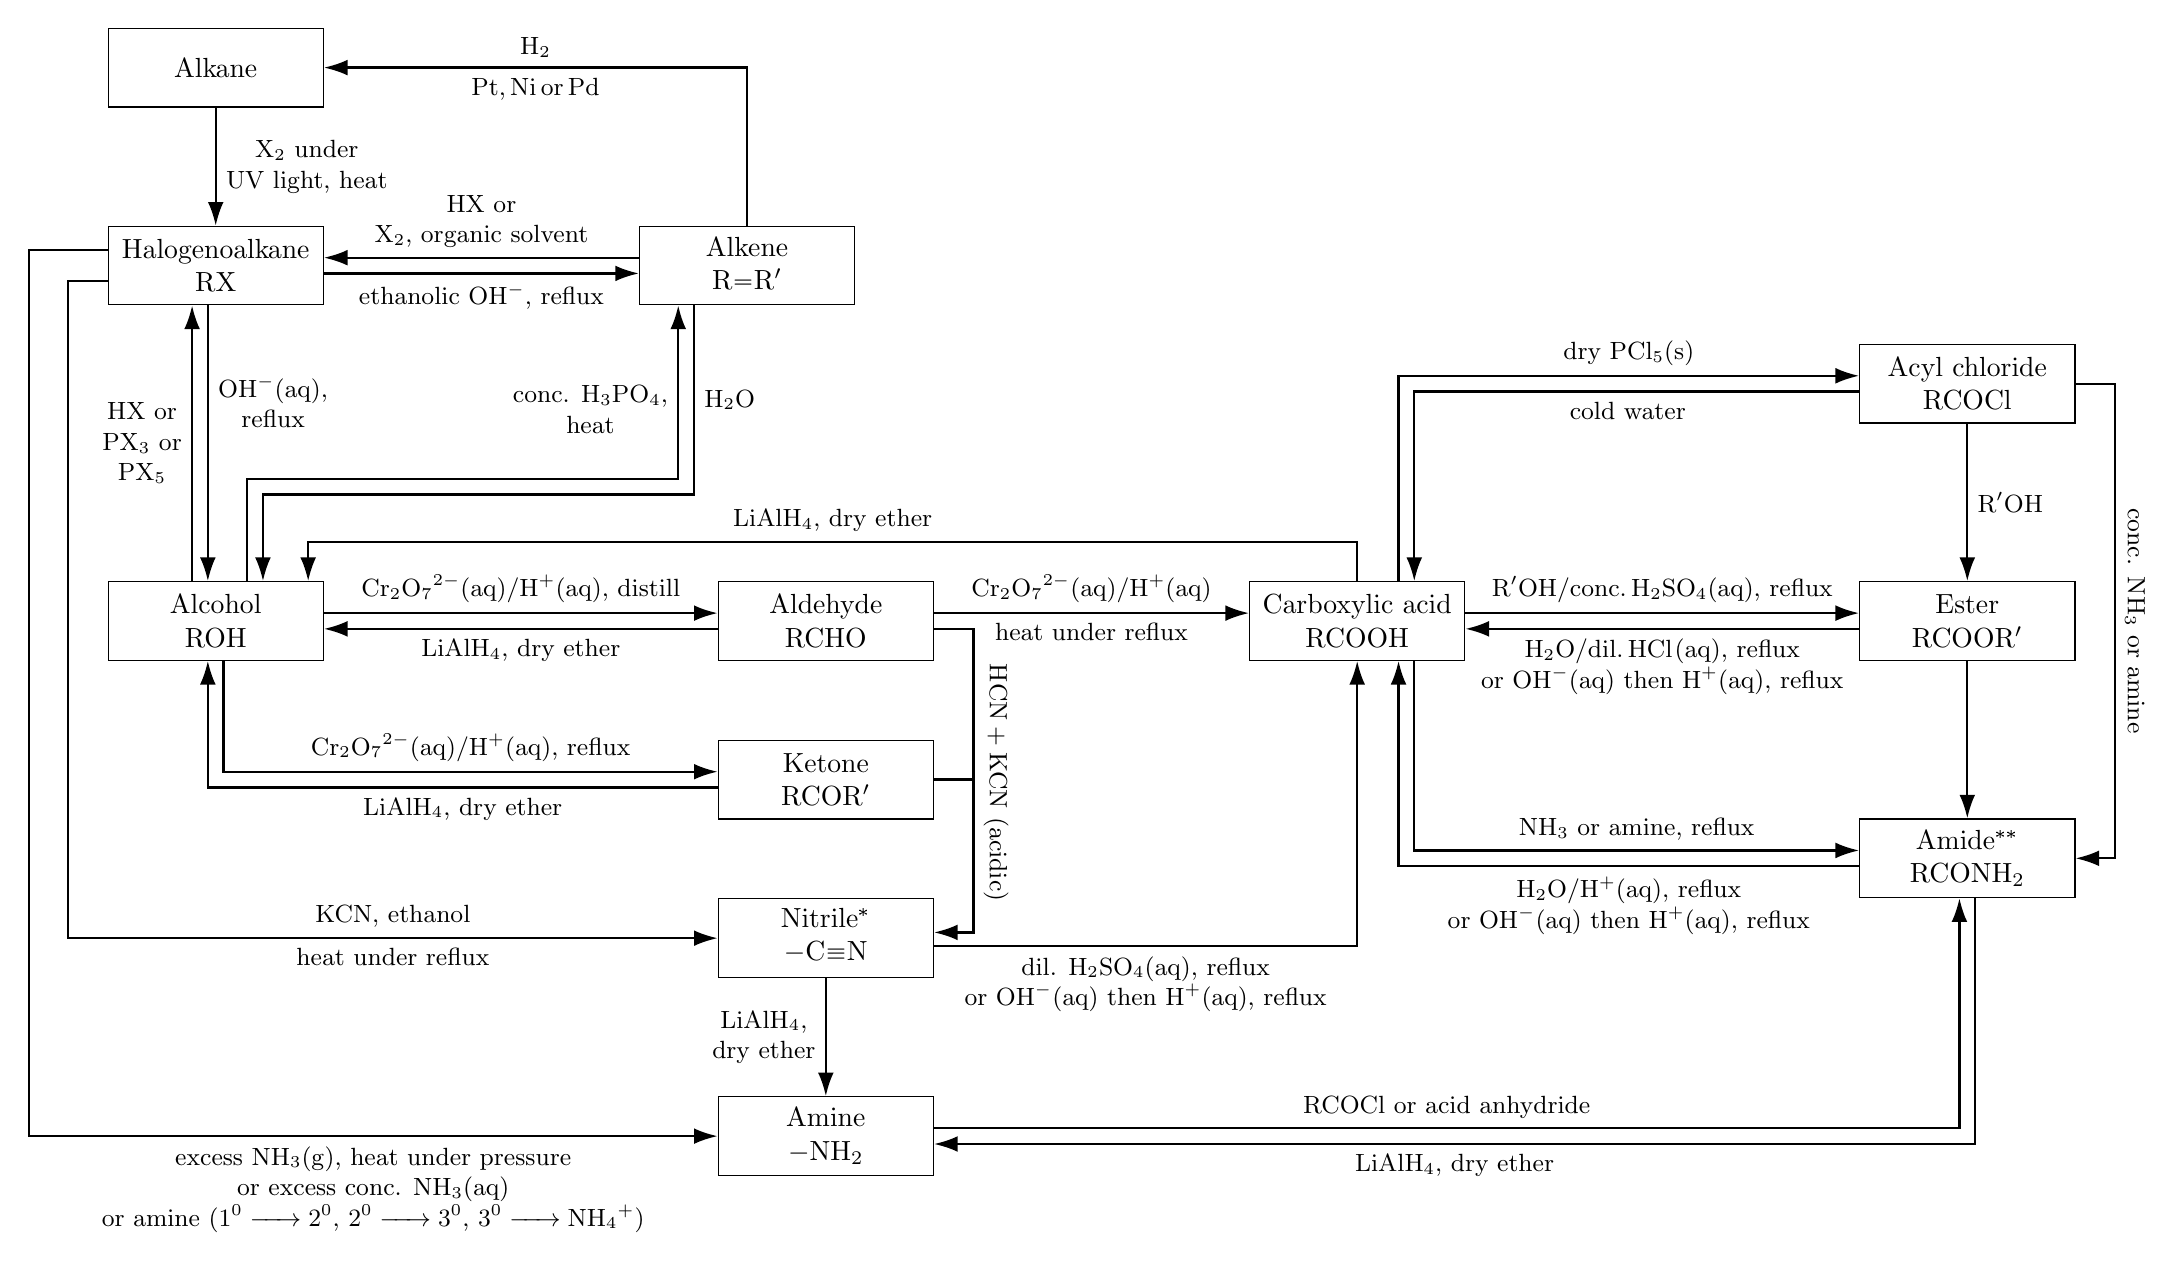
\begin{tikzpicture}[node distance=1cm]
\node (alkane) [rect] { Alkane };
\node (haloalkane) [rect, below=of alkane, yshift=-.5cm] { Halogenoalkane\\$\ce{RX}$ };
\node (alkene) [rect, right=of haloalkane, xshift=3cm] { Alkene\\$\ce{R=R{'}}$ };
\node (alcohol) [rect, below=of haloalkane, yshift=-2.5cm] { Alcohol\\$\ce{ROH}$};
\node (aldehyde) [rect, right=of alcohol, xshift=4cm] { Aldehyde\\$\ce{RCHO}$ };
\node (carboxylic) [rect, right=of aldehyde, xshift=3cm] { Carboxylic acid\\$\ce{RCOOH}$ };
\node (ketone) [rect, below=of aldehyde] { Ketone\\$\ce{RCOR{'}}$ };
\node (nitrile) [rect, below=of ketone] { Nitrile\footnotemark[1]\\$\ce{-C#N}$ };
\node (amine) [rect, below=of nitrile, yshift=-.5cm] { Amine\\$\ce{-NH2}$};
\node (ester) [rect, right=of carboxylic, xshift=4cm] { Ester\\$\ce{RCOOR{'}}$ };
\node (acyl) [rect, above=of ester, yshift=1cm] { Acyl chloride\\$\ce{RCOCl}$ };
\node (amide) [rect, below=of ester, yshift=-1cm] { Amide\footnotemark[7]\\$\ce{RCONH2}$};

% alkene -> alkane
\draw [arrow] (alkene.north) |- node[above, near end] {$\ce{H2}$} node[below, near end] {$\ce{Pt, Ni or Pd
}$} (alkane.east);

% alkane <-> halo
\draw [arrow] (alkane.south) -- node[right, midway, align=center] {$\ce{X2}$ under\\UV light, heat} (haloalkane.north);

% alkene <-> halo
\draw [arrow] ([yshift=1mm]alkene.west) -- node[above, midway, align=center] {$\ce{HX}$ or\\$\ce{X2}$, organic solvent} ([yshift=1mm]haloalkane.east);
\draw [arrow] ([yshift=-1mm]haloalkane.east) -- node[below, midway, align=center] {ethanolic $\ce{OH^-}$, reflux} ([yshift=-1mm]alkene.west);

% alkene <-> alcohol
\draw [arrow] ([xshift=4mm]alcohol.north) -- ++(0,1.3) -| node[left, pos=0.7, align=center] {conc. $\ce{H3PO4}$,\\heat} ([xshift=5mm]alkene.south west);
\draw [arrow] ([xshift=7mm]alkene.south west) -- node[right, pos=0.5] {$\ce{H2O}$} ++(0,-2.4) -| ([xshift=6mm]alcohol.north);

% halo <-> alcohol
\draw [arrow] ([xshift=-3mm]alcohol.north) -- node[left, midway, align=center]{$\ce{HX}$ or\\$\ce{PX3}$ or\\$\ce{PX5}$} ([xshift=-3mm]haloalkane.south);
\draw [arrow] ([xshift=-1mm]haloalkane.south) -- node[right, pos=0.35, align=center]{$\ce{OH^-(aq)}$,\\reflux} ([xshift=-1mm]alcohol.north);

% alcohol <-> aldehyde
\draw [arrow] ([yshift=1mm]alcohol.east) -- node[above] {$\ce{Cr2O7^2-(aq)/H+(aq)}$, distill} ([yshift=1mm]aldehyde.west);
\draw [arrow] ([yshift=-1mm]aldehyde.west) -- node[below] {$\ce{LiAlH4}$, dry ether} ([yshift=-1mm]alcohol.east);

% aldehyde -> carboxylic
\draw [arrow] ([yshift=1mm]aldehyde.east) -- node[above] {$\ce{Cr2O7^2-(aq)/H+(aq)}$} node[below] {heat under reflux} ([yshift=1mm]carboxylic.west);

% carboxylic -> alcohol
\draw [arrow] (carboxylic.north) -- +(0,0.5) -| node[above, pos=0.25] {$\ce{LiAlH4}$, dry ether} ([xshift=-2mm]alcohol.north east);

% alcohol <-> ketone
\draw [arrow] ([xshift=1mm]alcohol.south) |- node[above, pos=0.75] {$\ce{Cr2O7^2-(aq)/H+(aq)}$, reflux} ([yshift=1mm]ketone.west);
\draw [arrow] ([yshift=-1mm]ketone.west) -| node[below, pos=0.25] {$\ce{LiAlH4}$, dry ether} ([xshift=-1mm]alcohol.south);

% carbonyl -> nitrile
\draw [line] ([yshift=-1mm]aldehyde.east) -| ([xshift=.5cm]ketone.east);
\draw [arrow] (ketone.east) -- ++(0.5,0) |- node[above,rotate=270,pos=0.01] { $\ce{HCN + KCN}$ (acidic)} ([yshift=1mm]nitrile);

% halo -> nitrile
\draw [arrow] ([yshift=-2mm]haloalkane.west) -- ++(-0.5,0) |- node[above, pos=0.75] {$\ce{KCN}$, ethanol} node[below, pos=0.75] {heat under reflux} (nitrile.west);

% halo -> amine
\draw [arrow] ([yshift=2mm]haloalkane.west) -- ++(-1,0) |- node[below, pos=0.75, align=center] {excess $\ce{NH3(g)}$, heat under pressure\\or excess conc. $\ce{NH3(aq)}$\\or amine ($1^0\ce{->}2^0$, $2^0\ce{->}3^0$, $3^0\ce{-> NH4+}$)} (amine.west);

% nitrile -> carboxylic
\draw [arrow] ([yshift=-1mm]nitrile.east) -| (carboxylic.south) node[below, pos=0.25, align=center]{ dil. $\ce{H2SO4(aq)}$, reflux\\or $\ce{OH^-(aq)}$ then $\ce{H^+(aq)}$, reflux };

% nitrile -> amine
\draw [arrow] (nitrile) -- node[left, midway, align=center] {$\ce{LiAlH4}$,\\dry ether} (amine);

% carboxylic <-> ester
\draw [arrow] ([yshift=1mm]carboxylic.east) -- node[above]{ $\ce{R{'}OH{/conc.} H2SO4(aq)}$, reflux } ([yshift=1mm]ester.west);
\draw [arrow] ([yshift=-1mm]ester.west) -- node[below, align=center]{$\ce{H2O{/dil.} HCl(aq)}$, reflux\\or $\ce{OH^-(aq)}$ then $\ce{H^+(aq)}$, reflux} ([yshift=-1mm]carboxylic.east);

% carboxylic <-> acyl chloride
\draw [arrow] ([xshift=+5.25mm]carboxylic.north) |- node[above, pos=0.75]{ dry $\ce{PCl5(s)}$ }([yshift=1mm]acyl.west);
\draw [arrow] ([yshift=-1mm]acyl.west) -| node[below, pos=0.26]{ cold water } ([xshift=+7.25mm]carboxylic.north);

% carboxylic <-> amide
\draw [arrow] ([xshift=+7.25mm]carboxylic.south) |- node[above, pos=0.75]{ $\ce{NH3}$ or amine, reflux } ([yshift=1mm]amide.west);
\draw [arrow] ([yshift=-1mm]amide.west) -| node[below, pos=0.25, align=center]{$\ce{H2O{/}H+(aq)}$, reflux\\or $\ce{OH^-(aq)}$ then $\ce{H^+(aq)}$, reflux} ([xshift=+5.25mm]carboxylic.south);

% acyl chloride -> amide
\draw [arrow] (acyl.east) --++(0.5,0) |- node[above,rotate=270,pos=0.25]{ conc. $\ce{NH3}$ or amine } (amide.east);

% acyl chloride -> ester
\draw [arrow] (acyl.south) -- node[right]{ $\ce{R{'}OH}$ } (ester.north);

% ester -> amide
\draw [arrow] (ester.south) -- (amide.north);

% amide <-> amine
\draw [arrow] ([yshift=1mm]amine.east) -| node[above, pos=.25]{$\ce{RCOCl}$ or acid anhydride} ([xshift=-1mm]amide.south);
\draw [arrow] ([xshift=1mm]amide.south) |- node[below, pos=.75]{$\ce{LiAlH4}$, dry ether} ([yshift=-1mm]amine.east);

\end{tikzpicture}

\footnotetext[1]{Carbonyl compound reacts to form {
    \setchemfig{atom sep=2.5em}
    \chemfig{R-CH(-[2]OH)-C~N}
} (hydroxynitrile/cyanohydrin)}
\footnotetext[7]{Amide$\ce{<-->}$carboxylic acid is rarely used and out of syllabus. Use of acyl chloride is more common and practical}
\pagestyle{empty} % remove page number
\end{document}